\documentclass[twoside]{article}
\setlength{\oddsidemargin}{0 in}
\setlength{\evensidemargin}{0 in}
\setlength{\topmargin}{-0.6 in}
\setlength{\textwidth}{6.5 in}
\setlength{\textheight}{8.5 in}
\setlength{\headsep}{0.75 in}
\setlength{\parindent}{0 in}
\setlength{\parskip}{0.1 in}

\usepackage{url}
\usepackage{titlesec}
\setcounter{secnumdepth}{3}
\usepackage{palatino}
\usepackage{marginnote}
\usepackage{multirow}
\usepackage{easybmat,bigdelim,arydshln}
\usepackage[authoryear,round]{natbib}
\usepackage{amssymb,amsmath,amsthm,amsfonts}
\usepackage{mathtools}
%\usepackage{nicematrix}
\usepackage{arydshln}
\usepackage{caption}
\usepackage{hyperref}
\usepackage{tcolorbox}
\tcbuselibrary{skins, breakable, theorems}
\usepackage{newpxtext,newpxmath}
\usepackage{longtable}
\usepackage{enumitem}
\makeatletter

\let\bar\overline

\setlist[itemize]{topsep=0pt,leftmargin=10pt,itemsep=-0.2em}
\usepackage{xcolor}
\usepackage{tikz}
\usepackage{pgfplots}
\pgfplotsset{compat = newest}
\usetikzlibrary{patterns,decorations.pathreplacing,decorations.markings,fit,shapes.geometric,angles,quotes,arrows}
\usepgfplotslibrary{fillbetween}

\usepackage{ifthen}
\usepackage{tikz-3dplot}

\pgfdeclarelayer{ft}
\pgfdeclarelayer{bg}
\pgfsetlayers{bg,main,ft}

\hypersetup{
    colorlinks,
    citecolor=red,
    filecolor=black,
    linkcolor=violet,
    urlcolor=blue
}

\definecolor{myblue}{cmyk}{1,.72,0,.38}
\definecolor{mypurple}{cmyk}{.57,1,0,.58}
\definecolor{myred}{cmyk}{0,.88,.88,.58}
\definecolor{mygreen}{cmyk}{1,0,.69,.66}
\definecolor{myorange}{cmyk}{0,.58,100,.20}
\definecolor{glaucous}{rgb}{0.38, 0.51, 0.71}

\makeatletter
\renewcommand{\thefigure}{\thesection.\arabic{figure}}
\newtheoremstyle{indented}
  {3pt}% space before
  {3pt}% space after
  {\addtolength{\@totalleftmargin}{3.5em}
   \addtolength{\linewidth}{-3.5em}
   \parshape 1 3.5em \linewidth}% body font
  {}% indent
  {\bfseries}% header font
  {.}% punctuation
  {.5em}% after theorem header
  {}% header specification (empty for default)
\makeatother

\newcommand{\ind}{\perp\!\!\!\perp}

\theoremstyle{definition}
\newtheorem{defin}{Definition}[section] % Creates a new counter, number within section
\newtheorem{prt}[defin]{Remark} 
\newtheorem{prts}[defin]{Remarks} % Again share defin's counter
\newtheorem{exmp}[defin]{Example} % etc.
\newtheorem{exmps}[defin]{Examples}
\newtheorem*{note}{Note}
\tcbuselibrary{theorems}

% use counter*=defin to make each tcbtheorem share defin's counter

\newtcbtheorem[use counter*=defin, number within=section]{definition}{Definition}{enhanced, breakable,
    colback = white, colframe = red!55!black, colbacktitle = red!55!black, attach boxed title to top left = {yshift = -2.5mm, xshift = 3mm}, boxed title style = {sharp corners},fonttitle=\bfseries}{def}

\newtcbtheorem[use counter*=defin, number within=section]{theorem}{Theorem}{enhanced, breakable,
    colback = white, colframe = blue!45!black, colbacktitle = blue!45!black, attach boxed title to top left = {yshift = -2.5mm, xshift = 3mm}, boxed title style = {sharp corners},fonttitle=\bfseries}{thm}
    
\newtcbtheorem[use counter*=defin, number within=section]{proposition}{Proposition}{enhanced, breakable,
    colback = white, colframe = teal, colbacktitle = teal, attach boxed title to top left = {yshift = -2.5mm, xshift = 3mm}, boxed title style = {sharp corners},fonttitle=\bfseries}{prop}

\newtcbtheorem[use counter*=defin, number within=section]{lemma}{Lemma}{enhanced, breakable,
    colback = white, colframe = orange!80!black, colbacktitle = orange!80!black, attach boxed title to top left = {yshift = -2.5mm, xshift = 3mm}, boxed title style = {sharp corners},fonttitle=\bfseries}{lemma}

\newtcbtheorem[use counter*=defin, number within=section]{example}{Example}{enhanced, breakable,
    colback = white, colframe = yellow!60!black, colbacktitle = yellow!60!black, attach boxed title to top left = {yshift = -2.5mm, xshift = 3mm}, boxed title style = {sharp corners},fonttitle=\bfseries}{exmp}

\newtcbtheorem[use counter*=defin, number within=section]{assumption}{Assumption}{enhanced, breakable,
    colback = white, colframe = violet!60!white, colbacktitle = violet!60!white, attach boxed title to top left = {yshift = -2.5mm, xshift = 3mm}, boxed title style = {sharp corners},fonttitle=\bfseries}{assump}

\newtcbtheorem[use counter*=defin, number within=section]{algorithm}{Algorithm}{enhanced, breakable,
    colback = white, colframe = green!55!black, colbacktitle = green!55!black, attach boxed title to top left = {yshift = -2.5mm, xshift = 3mm}, boxed title style = {sharp corners},fonttitle=\bfseries}{algm}
%\newtcolorbox{example}[1]{enhanced, breakable, colback = white, colframe = orange!85!black, colbacktitle = orange!85!black, attach boxed title to top left = {yshift = -2.5mm, xshift = 3mm}, boxed title style = {sharp corners},fonttitle=\bfseries, title={Example: #1}}

\newtcbox{\myhl}[1][white]
  {on line, arc = 0pt, outer arc = 0pt,
    colback = #1!20!white, colframe = #1!50!black,
    boxsep = 0pt, left = 1pt, right = 1pt, top = 1pt, bottom = 1pt, boxrule = 0pt, bottomrule =0pt, toprule =0pt}
    
\newtcbox{\myhlrule}[1][white]
  {on line, arc = 0pt, outer arc = 0pt,
    colback = #1!20!white, colframe = #1!50!black,
    boxsep = 0pt, left = 1pt, right = 1pt, top = 1pt, bottom = 1pt, boxrule = 0pt, bottomrule =0.5pt, toprule =0.5pt}
%
% The following commands set up the lecnum (lecture number)
% counter and make various numbering schemes work relative
% to the lecture number.
%
\newcounter{lecnum}
\renewcommand{\thepage}{\thelecnum-\arabic{page}}
\renewcommand{\thesection}{\thelecnum.\arabic{section}}
\renewcommand{\theequation}{\thelecnum.\arabic{equation}}
\renewcommand{\thefigure}{\thelecnum.\arabic{figure}}
\renewcommand{\thetable}{\thelecnum.\arabic{table}}

\newcommand{\sidenotes}[1]{\marginnote{\raggedright\scriptsize#1}}
%
% The following macro is used to generate the header.
%
\newcommand{\lecture}[6]{
   \pagestyle{myheadings}
   \thispagestyle{plain}
   \newpage
   \setcounter{lecnum}{#1}
   \setcounter{page}{1}
   \noindent
   \begin{center}
   \framebox{
      \vbox{\vspace{2mm}
    \hbox to 6.28in { {\bf Econometrics
	\hfill \today} }
       \vspace{4mm}
       \hbox to 6.28in { {\Large \hfill Topic #1: #2  \hfill} }
       \vspace{2mm}
       \hbox to 6.28in { {\it #3 \hfill by #4} }
      \vspace{2mm}}
   }
   \end{center}
   \markboth{Week #1: #2}{Week #1: #2}

   {\bf Key points}: {#5}

   {\bf Disclaimer}: {\it #6}
   \vspace*{4mm}
}
%

\tikzset{-stealth-/.style={decoration={
  markings,
  mark=at position #1 with {\arrow{stealth}}},postaction={decorate}}}

  \tikzset{tangent/.style={
    decoration={
        markings,% switch on markings
        mark=
            at position #1
            with
            {
                \coordinate (tangent point-\pgfkeysvalueof{/pgf/decoration/mark info/sequence number}) at (0pt,0pt);
                \coordinate (tangent unit vector-\pgfkeysvalueof{/pgf/decoration/mark info/sequence number}) at (1,0pt);
                \coordinate (tangent orthogonal unit vector-\pgfkeysvalueof{/pgf/decoration/mark info/sequence number}) at (0pt,1);
            }
    },
    postaction=decorate
},
use tangent/.style={
    shift=(tangent point-#1),
    x=(tangent unit vector-#1),
    y=(tangent orthogonal unit vector-#1)
},
use tangent/.default=1}

\tikzstyle{terminator} = [rectangle, draw, thick, text centered, rounded corners, minimum height=2em]
\tikzstyle{process} = [rectangle, draw, thick, text centered, minimum height=2em]
\tikzstyle{decision} = [diamond, draw, thick, text centered, minimum width=3cm, minimum height=0.5cm]
\tikzstyle{data}=[trapezium, draw, thick, text centered, trapezium left angle=60, trapezium right angle=120, minimum height=2em]
\tikzstyle{arrow} = [thick,->,>=stealth]

\begin{document}
\lecture{12}{Non-convex Learning}{}{Sai Zhang}{$L$-0 penalty is the best choice, but mostly computationally infeasible. Concave penalty (such as SCAD) works well with high dimensional problems.}{The note is built on Prof. \hyperlink{http://faculty.marshall.usc.edu/jinchi-lv/}{Jinchi Lv}'s lectures of the course at USC, DSO 607, High-Dimensional Statistics and Big Data Problems.}

\section{L0 Penalized Likelihood}
Consider the model selection problem of choosing a parameter vector $\boldsymbol{\theta}$ that maximizes the penalized likelihood 
\begin{equation}\label{eq:l0}
    \mathcal{L}_n(\boldsymbol{\theta}) - \lambda \lVert \boldsymbol{\theta} \rVert _0
\end{equation}
where the $L_0$-norm $\lVert c\dot \rVert _0$ denotes the \myhl[myblue]{\textbf{the number of nonzero components}}, and $\lambda\geq 0$ is still the regularization parameter.

The $L_0-$penalized likelihood method is equivalent to \myhl[myred]{\textbf{the best subset selection}}
\begin{itemize}
    \item given $\lVert \boldsymbol{\theta}_0\rVert _0=m$, the solution to Problem \ref{eq:l0} is the \myhl[myblue]{\textbf{best subset}} that has the \textbf{\underline{largest}} maximum likelihood among all subsets of size $m$
    \item then, choose the model size $m$ among the $p$ size-$m$ best subsets ($1\leq m\leq p$) by maximizing \ref{eq:l0}
\end{itemize}
hence it's a combinatorial problem, computationally complex.

\paragraph*{$L_0$-Penalized Empirical Risk Minimization} More generally, consider a unified approach of $L_0-$penalized empirical risk minimization for variable selection:
\begin{equation}\label{eq:empirical-l0}
    \min_{\boldsymbol{\theta}\in\mathbb{R}^p}\left\{\hat{R}(\boldsymbol{\theta}) + \lambda\lVert \boldsymbol{\theta} \rVert _0 \right\}
\end{equation}
where $\hat{R}(\boldsymbol{\theta})$ is the empirical risk function, which could be of different forms
\begin{itemize}
    \item \underline{\textbf{negative log-likelihood loss}}: equivalent t $L_0$-penalized likelihood 
    \item \textbf{\underline{squared error (quadratic) loss}}: $L_0$-penalized least squares
    \item \underline{selection via \textbf{RSS} (residual sum of squares)}: for the adjusted $R^2$
    $$
    R^2_{\text{adj}} = 1-\frac{n-1}{n-d}\frac{RSS_d}{TSS}
    $$
    it's clear that $\max R^2_{\text{adj}}\Leftrightarrow \min\log\left(\frac{RSS_d}{n-d}\right)$, and since $\frac{RSS_d}{n}\simeq \sigma^2$, then $$ n\log \frac{RSS_d}{n-d}\simeq \frac{RSS_d}{\sigma^2} + d + n(\log \sigma^2 -1) $$ which shows that adjusted $R^2$ method is approximately equivalent to \ref{eq:empirical-l0} with $\lambda =1/2$
    \item \underline{\textbf{generalized corss-validation} (GCV)}, \underline{\textbf{corss-validation} (CV)}
    \item \underline{\textbf{risk inflation factor} (RIC)}: use $\lambda = \log p$, adjusting for the inflation of prediction risk caused by searching $p$ variables\footnote{The $\log p$ is, once again, from the fact that for Gaussian random variables $$ \max_{1\leq j\leq p}\lvert Z_i\rvert \simeq \sqrt{2\log p} $$ for $(Z_1,\cdots,Z_p)'\sim\mathcal{N}(0,\mathbf{I}_p)$}
    \item \underline{\textbf{AIC}} ($\lambda=1$), \underline{\textbf{BIC}} ($\lambda=\frac{\log n}{2}$)
\end{itemize}

\subsection{Properties of L0-Regularization Methods}
\paragraph*{\myhl[myred]{\textbf{risk bounds}}}
for model selection \citep{barron1999risk}: for a family of models $\left\{ S_m: m\in\mathcal{M}_p \right\}$, The penalty term generally takes the form of $$ \frac{\kappa L_m D_m}{n} $$ where 
    \begin{itemize}
        \item $\kappa$: a positive constant
        \item $D_m = \lvert S_m \rvert$: the model dimension, account for the difficulty to estimate \textbf{\underline{within}} the model $S_m$
        \item $L_m\geq 1$: a weight that satisfies: $\sum_{m\in \mathcal{M}_p}\exp(-L_mD_m)\leq 1$, accounting for the noise due to \textbf{\underline{the size}} of the list of models
    \end{itemize}
hence, in the linear model, the $L_0$-regularized estimator $\hat{\boldsymbol{\beta}}$ satisfies that 
$$
\mathbb{E}\left[ n^{-1}\lVert \mathbf{X}\hat{\boldsymbol{\beta}}- \mathbf{X}{\boldsymbol{\beta}}_0 \rVert^2_2 \right] \leq C \inf_{m\in \mathcal{M}_p}\left\{ \min_{\boldsymbol{\beta}\in\text{model }S_m} \left[ n^{-1}\lVert \mathbf{X}{\boldsymbol{\beta}}- \mathbf{X}{\boldsymbol{\beta}}_0 \rVert^2_2 \right] + \frac{\kappa L_m D_m}{n}\right\}
$$
where \textit{\underline{\textbf{the tradeoff}}}: approximation error $ n^{-1}\lVert \mathbf{X}\hat{\boldsymbol{\beta}}- \mathbf{X}{\boldsymbol{\beta}}_0 \rVert^2_2 $, and the cost of searching $\frac{\kappa L_m D_m}{n}$

\paragraph*{\myhl[myred]{\textbf{computational complexity}}} $L_0-$regularization methods are appealing w.r.t. risk properties, but in high-dimensional settings, the computation is infeasible (combinatorial), and discontinuous, non-convex penalty function $\lambda \lVert \boldsymbol{\beta}\rVert _0$

\subsection{Generalizations of L0-Regularization Methods}
Consider continuous or convex relaxation of the $L_0$-regularization method 
\begin{equation}\label{eq:relaxed-l0}
    \min_{\boldsymbol{\beta}\in\mathbb{R}^p} \left\{ \hat{R}(\boldsymbol{\beta}) + \sum^p_{j=1}p_{\lambda}\left(\lvert \beta_j \rvert\right) \right\}
\end{equation}
where, as in Problem \ref{eq:empirical-l0}
\begin{itemize}
    \item $\hat{R}(\boldsymbol{\beta})$: the empirical risk function 
    \item $p_{\lambda}(t),t\geq 0$: the nonnegative penalty function indexed by the regularization parameter $\lambda \geq 0$ with $p_{\lambda}(0)=0$
\end{itemize}

\paragraph*{Choices of penalty function} In general, the choices of penalty function can be up for the researchers to decide. \citet{fan2001variable} proposed 3 criteria for the selection of penalty function $p_\lambda(t)$
\begin{itemize}
    \item \myhl[myblue]{\textbf{Sparsity}}: $p'_{\lambda}(0+)>0$, sets small coefficients to 0, for \textit{variable selection} and \textit{reducing model complexity}
    \item \myhl[myblue]{\textbf{Approximate unbiasedness}}: nearly unbiased, especially when the true coefficient $\beta_j$ is large
    \item \myhl[myblue]{\textbf{Continuity}}: continuous in data to reduce instability in model selection
\end{itemize}
To elaborate the 3 criterion, consider a class of penalty function, $L_q$-penalty 
$$
p_{\lambda}(t) = \lambda t^q, t\geq 0 \Rightarrow p'_{\lambda}(t) = \lambda qt^{q-1}
$$
then we can compare
\begin{center}
    \begin{tabular}{ r|ccc } 
        & Sparsity & Approx. unbiasedness & Continuity \\
     \hline
     $0<q<1$ & Y & Y & N \\
     $q=1$ & Y & N & Y \\
     $1<q\leq 2$ & N & N & Y \\
     \hline
    \end{tabular}
\end{center}
this class of penalty functions includes:
\begin{itemize}
    \item $q=0$: $L_0-$ regression (best subset selection)
    \item $q=1$: Lasso
    \item $q=2$: Ridge
    \item $0<q<2$: Bridge estimator
\end{itemize}

\section{High Dimensional Variable Selection}
For a generalized linear model 
$$
f_n(\mathbf{y};\mathbf{X},\boldsymbol{\beta}) = \prod_{i=1}^n \left\{ c(y_i)\exp\left( \frac{y_i\theta_i-b(\theta_i)}{\phi} \right) \right\}
$$
where $\boldsymbol{\theta}=(\theta_1,\cdots,\theta_n)' = \mathbf{X}\boldsymbol{\beta}$ is the \myhl[myred]{\textbf{natural parameter vector}}, which can a very challenging problem. Instead of the penalized least squares, now we examine \myhl[myred]{\textbf{penalized likelihood}}
\begin{equation}\label{eq:penal_likelihood}
    \max_{\boldsymbol{\beta}\in\mathbb{R}^p}\mathcal{L}_n(\boldsymbol{\beta}) -\sum^p_{j=1}p_{\lambda_n}\left( \lvert \beta_j \rvert \right)
\end{equation}
where $\mathcal{L}_n(\boldsymbol{\beta}) = n^{-1} \left[ \mathbf{y}'\mathbf{X}\boldsymbol{\beta} - \mathbf{1}'\mathbf{b}(\mathbf{X}\boldsymbol{\beta}) \right]$ is the \textit{\underline{affine transformation}} of log-likelihood, $$ \mathbf{b}(\boldsymbol{\theta})= \mathbf{b}(\mathbf{X}\boldsymbol{\beta}) = \left( b(\theta_1),\cdots,b(\theta_n) \right)'$$
So the natural question is, when can we find the solution to Problem \ref{eq:penal_likelihood}, s.t. $\mathrm{supp}(\hat{\boldsymbol{\beta}}) = \mathrm{supp}(\boldsymbol{\beta}_0)$, that is, covering exactly the ture underlying sparse model?

\section{Penalized Likelihood with Concave Penalties}
$$
    \max_{\boldsymbol{\beta}\in\mathbb{R}^p}\mathcal{L}_n(\boldsymbol{\beta}) -\sum^p_{j=1}p_{\lambda_n}\left( \lvert \beta_j \rvert \right)
$$
where $\mathcal{L}_n(\boldsymbol{\beta}) = n^{-1} \left[ \mathbf{y}'\mathbf{X}\boldsymbol{\beta} - \mathbf{1}'\mathbf{b}(\mathbf{X}\boldsymbol{\beta}) \right]$, and $p_{\lambda}(\cdot)$ is a concave penalty function. Let $\rho(t;\lambda)=\lambda^{-1}p_{\lambda}(t),t\geq 0$, we aim for penalty functions that satisfy
\begin{itemize}
    \item $\rho(t)$ is \myhl[myred]{\textbf{increasing and concave}} in $t$
    \item $\rho'(t)$ is \myhl[myred]{\textbf{continuous}} with $\rho'(0+)>0$
    \item if $\rho(t)$ depends on $\lambda$, $\rho'(t;\lambda)$ is \myhl[myred]{\textbf{increasing} in $\lambda$} and $\rho'(0_+;\lambda)$ is \myhl[myred]{\textbf{independent}} of $\lambda$
\end{itemize}

Here are some notations
\begin{itemize}
    \item Moment property: $k-$th component-wise derivative corresponds to $k-$th moment
    \begin{itemize}
        \item $\boldsymbol{\mu}(\boldsymbol{\theta}) = (b'(\theta_1),\cdots,b'(\theta_n))'$: $\mathbb{E}(\mathbf{y})$
        \item $\boldsymbol{\Sigma}(\boldsymbol{\theta}) = \mathrm{diag}\left\{ b''(\theta_1),\cdots,b''(\theta_n) \right\} $
    \end{itemize}
    \item local concavity of $\rho$ at $\mathbf{v}=(v_1,\cdots,v_q)'\in\mathbb{R}^q$, with $\lVert \mathbf{v} \rVert _0 = q$, that is 
    $$ 
    \kappa(\rho;\mathbf{v}) = \lim_{\epsilon\rightarrow 0_+} \max_{1\leq j\leq q} \sup_{t_1<t_2\in (|v_j|-\epsilon,|v_j|+\epsilon)} - \frac{\rho'(t_2)-\rho'(t_1)}{t_2-t_1}
    $$
    if $\rho''(t)$ is continuous, this becomes
    $$
    \max_{1\leq j\leq q} -\rho''(|v_j|)
    $$
\end{itemize}
And the solution is given by the following theorem 
\begin{theorem}{Penalized Likelihood estimator}{penal_ll_est}
    $\hat{\boldsymbol{\beta}}$ is \textbf{strict \myhl[myblue]{local}} maximizer of penalized likelihood if
    \begin{align*}
        \mathbf{X}_1'\mathbf{y} - \mathbf{X}_1'\boldsymbol{\mu}(\boldsymbol{\hat{\theta}})-n\lambda_n \mathrm{sign}(\hat{\boldsymbol{\beta}}_1)\circ \rho'(\lvert \hat{\boldsymbol{\beta}}_1 \rvert) &= \mathbf{0} \\
        \lVert (n\lambda_n)^{-1}\mathbf{X}_2'[\mathbf{y}-\boldsymbol{\mu}(\hat{\boldsymbol{\theta}})] \rVert _{\infty} &< \rho'(0_+) \\
        \lambda_{\min}\left[\mathbf{X}_1'\boldsymbol{\Sigma}(\hat{\boldsymbol{\theta}})\mathbf{X}_1\right] &> n\lambda_n \kappa(\rho;\hat{\boldsymbol{\beta}}_1)
    \end{align*}
    where $\circ$ is the component-wise multiplication, $\lambda_{\min}(\cdot)$ is the smallest eigenvalue.
\end{theorem}

\subsection{Global Optimality}
Theorem \ref{thm:penal_ll_est} gives the rule to find local maximizers, but what about global optimality?

\begin{proposition}{Global Optimality of Penalized Likelihood Estimator}{llest_global}
    Assume that $\mathbf{X}$ has rank $p$, and satisfies 
    $$
    \min_{\boldsymbol{\beta}\in \mathcal{L}_c} \lambda_{\min} \left[n^{-1} \mathbf{X}'\boldsymbol{\Sigma}(\mathbf{X}\boldsymbol{\beta})\mathbf{X} \right] \geq \kappa(p_{\lambda_n})
    $$
    where 
    \begin{itemize}
        \item NOT high-dimensional: $p\leq n$
        \item for some $c< \mathcal{L}_n (\mathbf{0})$, $$ \mathcal{L}_c = \left\{ \boldsymbol{\beta}\in \mathbb{R}^p: \mathcal{L}_n(\boldsymbol{\beta})\geq c \right\} $$ is a sublevel set of $-\mathcal{L}_n(\boldsymbol{\beta})$
        \item maximum concavity $$ \kappa(p_{\lambda}) = \sup_{t_1<t_2\in(0,\infty)}-\frac{p'_{\lambda}(t_2)-p'_{\lambda}(t_1)}{t_2-t_1} $$
    \end{itemize}
\end{proposition}

\subsection{SCAD penalty}

Now, consider a penalized likelihood model: \myhl[myblue]{\textbf{SCAD}} \citep[smoothly clipped
absolute deviation]{fan2001variable}
$$
\min_{\boldsymbol{\beta}} \lVert \mathbf{y}-\mathbf{X}\boldsymbol{\beta} \rVert^2_2 + p(\boldsymbol{\beta})
$$
where the derivative of the penalty function
$$
p_{\lambda}^{\text{SCAD}}(\beta_j) = \begin{cases}
    \lambda \lvert \beta_j  \rvert & \lvert \beta_j \rvert \leq \lambda \\
    -\left( \frac{\lvert \beta_j \rvert^2 - 2a\lambda \lvert \beta_j \rvert + \lambda^2}{2(a-1)} \right) & \lambda <\lvert \beta_j \rvert \leq a\lambda\\
    \frac{(a+1)\lambda^2}{2} & \lvert \beta_j \rvert > a\lambda
\end{cases}
$$
and its derivative
$$
p'(\boldsymbol{\beta}) = \lambda \left[ I(\boldsymbol{\beta} \leq \lambda) + \frac{(a\lambda - \boldsymbol{\beta})_+}{(a-1)\lambda} I(\boldsymbol{\beta}>\lambda) \right]
$$
the solution to SCAD penalty model is
$$
\hat{\beta}_j^{\text{SCAD}} = \begin{cases}
    (\lvert \hat{\beta}_j \rvert)_+\mathrm{sign}(\hat{\beta}_j) & \lvert \hat{\beta}_j \rvert< 2\lambda \\
    \frac{(a-1)\hat{\beta}_j-\mathrm{sign}(\hat{\beta}_j)a\lambda}{a-2} & 2\lambda < \lvert \hat{\beta}_j \rvert \leq a\lambda \\
    \hat{\beta}_j & \lvert \hat{\beta}_j \rvert> a\lambda
\end{cases}
$$
the SCAD penalty is continuously differentiable on $(-\infty,0)\cup (0,\infty)$, singular at $0$. SCAD has some great properties, one of them is robustness.
\begin{proposition}{Robustness of SCAD}{scad_robust}
    Assume that $\mathbf{X}$ has rank $p=s$, and $\exists c< \mathcal{L}_n(\mathbf{0})$ s.t. for some $c_0 > 0$
    $$
    \min_{\boldsymbol{\beta}\in \mathcal{L}_c} \lambda_{\min} \left[n^{-1} \mathbf{X}'\boldsymbol{\Sigma}(\mathbf{X}\boldsymbol{\beta})\mathbf{X} \right]\geq c_0
    $$
    then the SCAD penalized likelihood estimator $\hat{\boldsymbol{\beta}}^{\text{SCAD}}$ is the \textbf{global} maximizer and equals the oracle MLE $\boldsymbol{\beta}^*$, if $\hat{\boldsymbol{\beta}}^{\text{SCAD}}$ and 
    $$
    \min_{j=1}^p \lvert \hat{\beta}^{\text{SCAD}}_j \rvert > \left( a + \frac{1}{2c_0} \right) \lambda_n
    $$
\end{proposition}
Next, we extend this global optimality result to high-dimensional cases, where $p>n$
\begin{proposition}{Global Optimality, $p>n$}{scad_highdimen}
    On the union of all $s-$dimensional coordinate subspaces of $\mathbb{R}^p$
    \begin{itemize}
        \item Under Proposition \ref{prop:llest_global} for each $n\times 2s$ submatrix of $\mathbf{X}$, then the NCPMLE $\hat{\boldsymbol{\beta}}$ is a global maximizer on $\mathbb{S}_s$
        \item Under Proposition \ref{prop:scad_robust} for $n\times s$ submatrix of $\mathbf{X}$ formed by columns in $\mathrm{supp}(\boldsymbol{\beta}_0)$, the true model is $\delta$-identifiable for some $ \delta > \frac{(a+1)s\lambda^2_n}{2} $, and $\mathrm{supp}(\hat{\boldsymbol{\beta}}) = \mathrm{supp}(\boldsymbol{\beta}_0)$. Then the SCAD penalized likelihood estimator $\hat{\boldsymbol{\beta}}$ is the global maximizer on $\mathbb{S}_s$ and \textbf{equals} to the oracle MLE $\boldsymbol{\beta}^*$
    \end{itemize}
\end{proposition}

\subsection{Regularity Conditions for Concave Penalties}
The regularity conditions for concave penalty are
\begin{itemize}
    \item the true sub design matrix $\mathbf{X}_1$ should be well conditioned $$ \left\Vert \left[\mathbf{X}_1'\boldsymbol{\Sigma}(\boldsymbol{\theta}_0)\mathbf{X}_1\right]^{-1} \right\Vert _{\infty} = O(b_sn^{-1})$$
    \item A generalized version of the irrepresentable condition \begin{equation}\label{eq:generalized_ic}
        \left\Vert \mathbf{X}_2' \boldsymbol{\Sigma}(\boldsymbol{\theta}_0) \mathbf{X}_1 \left[\mathbf{X}_1'\boldsymbol{\Sigma}(\boldsymbol{\theta}_0)\mathbf{X}_1\right]^{-1} \right\Vert _{\infty} \leq \min \left\{ C\frac{\rho'(0+)}{\rho'(d_n)}, O(n^{\alpha_1})\right\}
    \end{equation}
    \item also $$\max_{\boldsymbol{\delta}\in\mathcal{N}_0}\max^p_{j=1} \lambda_{\max}\left[ \mathbf{X}_1' \mathrm{diag} \left\{ \lvert \mathbf{x}_j \rvert \circ \lvert \boldsymbol{\mu}''(\mathbf{X}_1\boldsymbol{\delta}) \rvert \right\} \mathbf{X}_1 \right] = O(n)$$
\end{itemize}
Here, $b_s \rightarrow \infty$ with $s=\lVert \boldsymbol{\beta}_0 \rVert _0 = O(n^{\alpha_0})$, $\alpha_1\in [0,1/2]$, $C\in(0,1)$, $\mathcal{N}_0 = \left\{ \boldsymbol{\delta}\in\mathbb{R}^s: \lVert \boldsymbol{\delta}-\boldsymbol{\beta}_1 \rVert _{\infty} \leq d_n \right\}$; $\alpha = \min(\frac{1}{2},2\gamma-\alpha_0)-\alpha_1$, $d_n\geq n^{-\gamma}\log n $ for some $\gamma \in (0, 1/2]$.

Notice that in a linear model, Condition \ref{eq:generalized_ic} becomes 
$$
\left\Vert \mathbf{X}_2' \mathbf{X}_1 \left(\mathbf{X}_1'\mathbf{X}_1\right)^{-1} \right\Vert _{\infty} \leq \min \left\{ C\frac{\rho'(0+)}{\rho'(d_n)}, O(n^{\alpha_1})\right\}
$$
\begin{itemize}
    \item For $L_1$ penalty, this becomes ($\rho'(0+)=\rho'(d_n)=1$) a \textbf{stronger} form of the irrepresentable condition $$ \left\Vert \mathbf{X}_2' \mathbf{X}_1 \left(\mathbf{X}_1'\mathbf{X}_1\right)^{-1} \right\Vert _{\infty} \leq C <1 $$, this speaks about the restrictive nature of $L_1$ penalty in higher dimensions
    \item For concave penalty, $\frac{\rho'(0+)}{\rho'(d_n)}$ \textbf{can grow} to $\infty$, hence, it is a much weaker condition: \myhl[myred]{\textbf{the flexibility}} of concave penalty.
\end{itemize}

\subsection{Properties of Concave Penalty}
Next, we establish the nonasymptotic weak oracle property for estimator with concave penalties.
\begin{theorem}{Nonasymptotic Weak Oracle Property}{nonasymp_weak_oracle}
    Under some regularity conditions, $s=o(n)$ and $\log p=O(n^{1-2\alpha})$, there exists a penalized likelihood estimator $\boldsymbol{\beta}$ s.t. for sufficiently large $n$, with probability of at least $$ 1-2\left[ sn^{-1}+(p-s)e^{-n^{1-2\alpha}\log n} \right] $$ $\hat{\boldsymbol{\beta}}$ satisfies 
    \begin{itemize}
        \item Sparsity: $\hat{\boldsymbol{\beta}}_2 =\mathbf{0}$
        \item $L_{\infty}$ loss: $\lVert \hat{\boldsymbol{\beta}}_1 -\boldsymbol{\beta}_1 \rVert _{\infty} = O(n^{-\gamma}log n)$
    \end{itemize}
\end{theorem}
This theorem shows that concave penalties can reduce biases of estimates. The $L_{\infty}$ estimation loss can de decomposed into $L_{\infty}\leq h_1 + h_2 + h_3$, $h_2 \sim b_s \lambda_s \frac{\rho'(d_n)}{\rho'(0+)}$. Theorem \ref{thm:nonasymp_weak_oracle} establishes nonasymptotic weak oracle property of penalized likelihood estimator with penalties, where dimensionality $p$ can grow non-polynomially with sample size $n$.

\begin{theorem}{Non-Concave Penalized Likelihood Estimator}{nonconcave_penal}
    Under some regularity conditions, $s\ll n$ and $\log p = O(n^{\alpha})$ for some $\alpha \in (0,1/2)$, there exists a strict local maximizer $\hat{\boldsymbol{\beta}}$ of penalized likelihood such that $that{\boldsymbol{\beta}}_2=\mathbf{0}$ with probability tending to 1 as $n\rightarrow \infty$ and $\lVert \hat{\boldsymbol{\beta}}-\boldsymbol{\beta}_0 \rVert _2=O_P(\sqrt{s}n^{-1/2})$.
\end{theorem}
These conditions are incompatible for $L_1$ penalty, suggesting that $L_1$ penalized likelihood estimator generally \textbf{cannot} achieve consistency rate $O_P(\sqrt{s}n^{-1/2})$ and \textbf{does not} have oracle property, when dimensionality $p$ is diverging with sample size $n$.

\begin{theorem}{Oracle Property of Non-Concave Penalty}{nonconcave_oracle}
    Under some regularity conditions and $s=o(n^{1/3})$, then with probability tending to 1 as $n\rightarrow \infty$, then non-concave penalized likelihood estimator $\hat{\boldsymbol{\beta}}$ in Theorem \ref{thm:nonconcave_penal} must satisfies 
    \begin{itemize}
        \item \textbf{Sparsity} $$\hat{\boldsymbol{\beta}}_2 =\mathbf{0}$$
        \item \textbf{Asymptotic normality} $$ \mathbf{A}_n \left[ \mathbf{X}_1' \boldsymbol{\Sigma}(\boldsymbol{\theta}_0)\mathbf{X}_1 \right]^{1/2}(\hat{\boldsymbol{\beta}}_1,\boldsymbol{\beta}_1) \xrightarrow{d} \mathcal{N}(\mathbf{0},\phi\mathbf{G}) $$
        where $\mathbf{A}_n$ is a $q\times s$ matrix s.t. $\mathbf{A}_n\mathbf{A}_n'\rightarrow \mathbf{G}$, and $\mathbf{G}$ is a $q\times q$ symmetric positive definite matrix.
    \end{itemize}
\end{theorem}

A simulation of SCAD versus Lasso is presented in Figure \ref{fig:SCADvsLasso}

\begin{figure}[ht]
    \centering
    \caption{Numercial Comparison: SCAD vs Lasso}\label{fig:SCADvsLasso}
    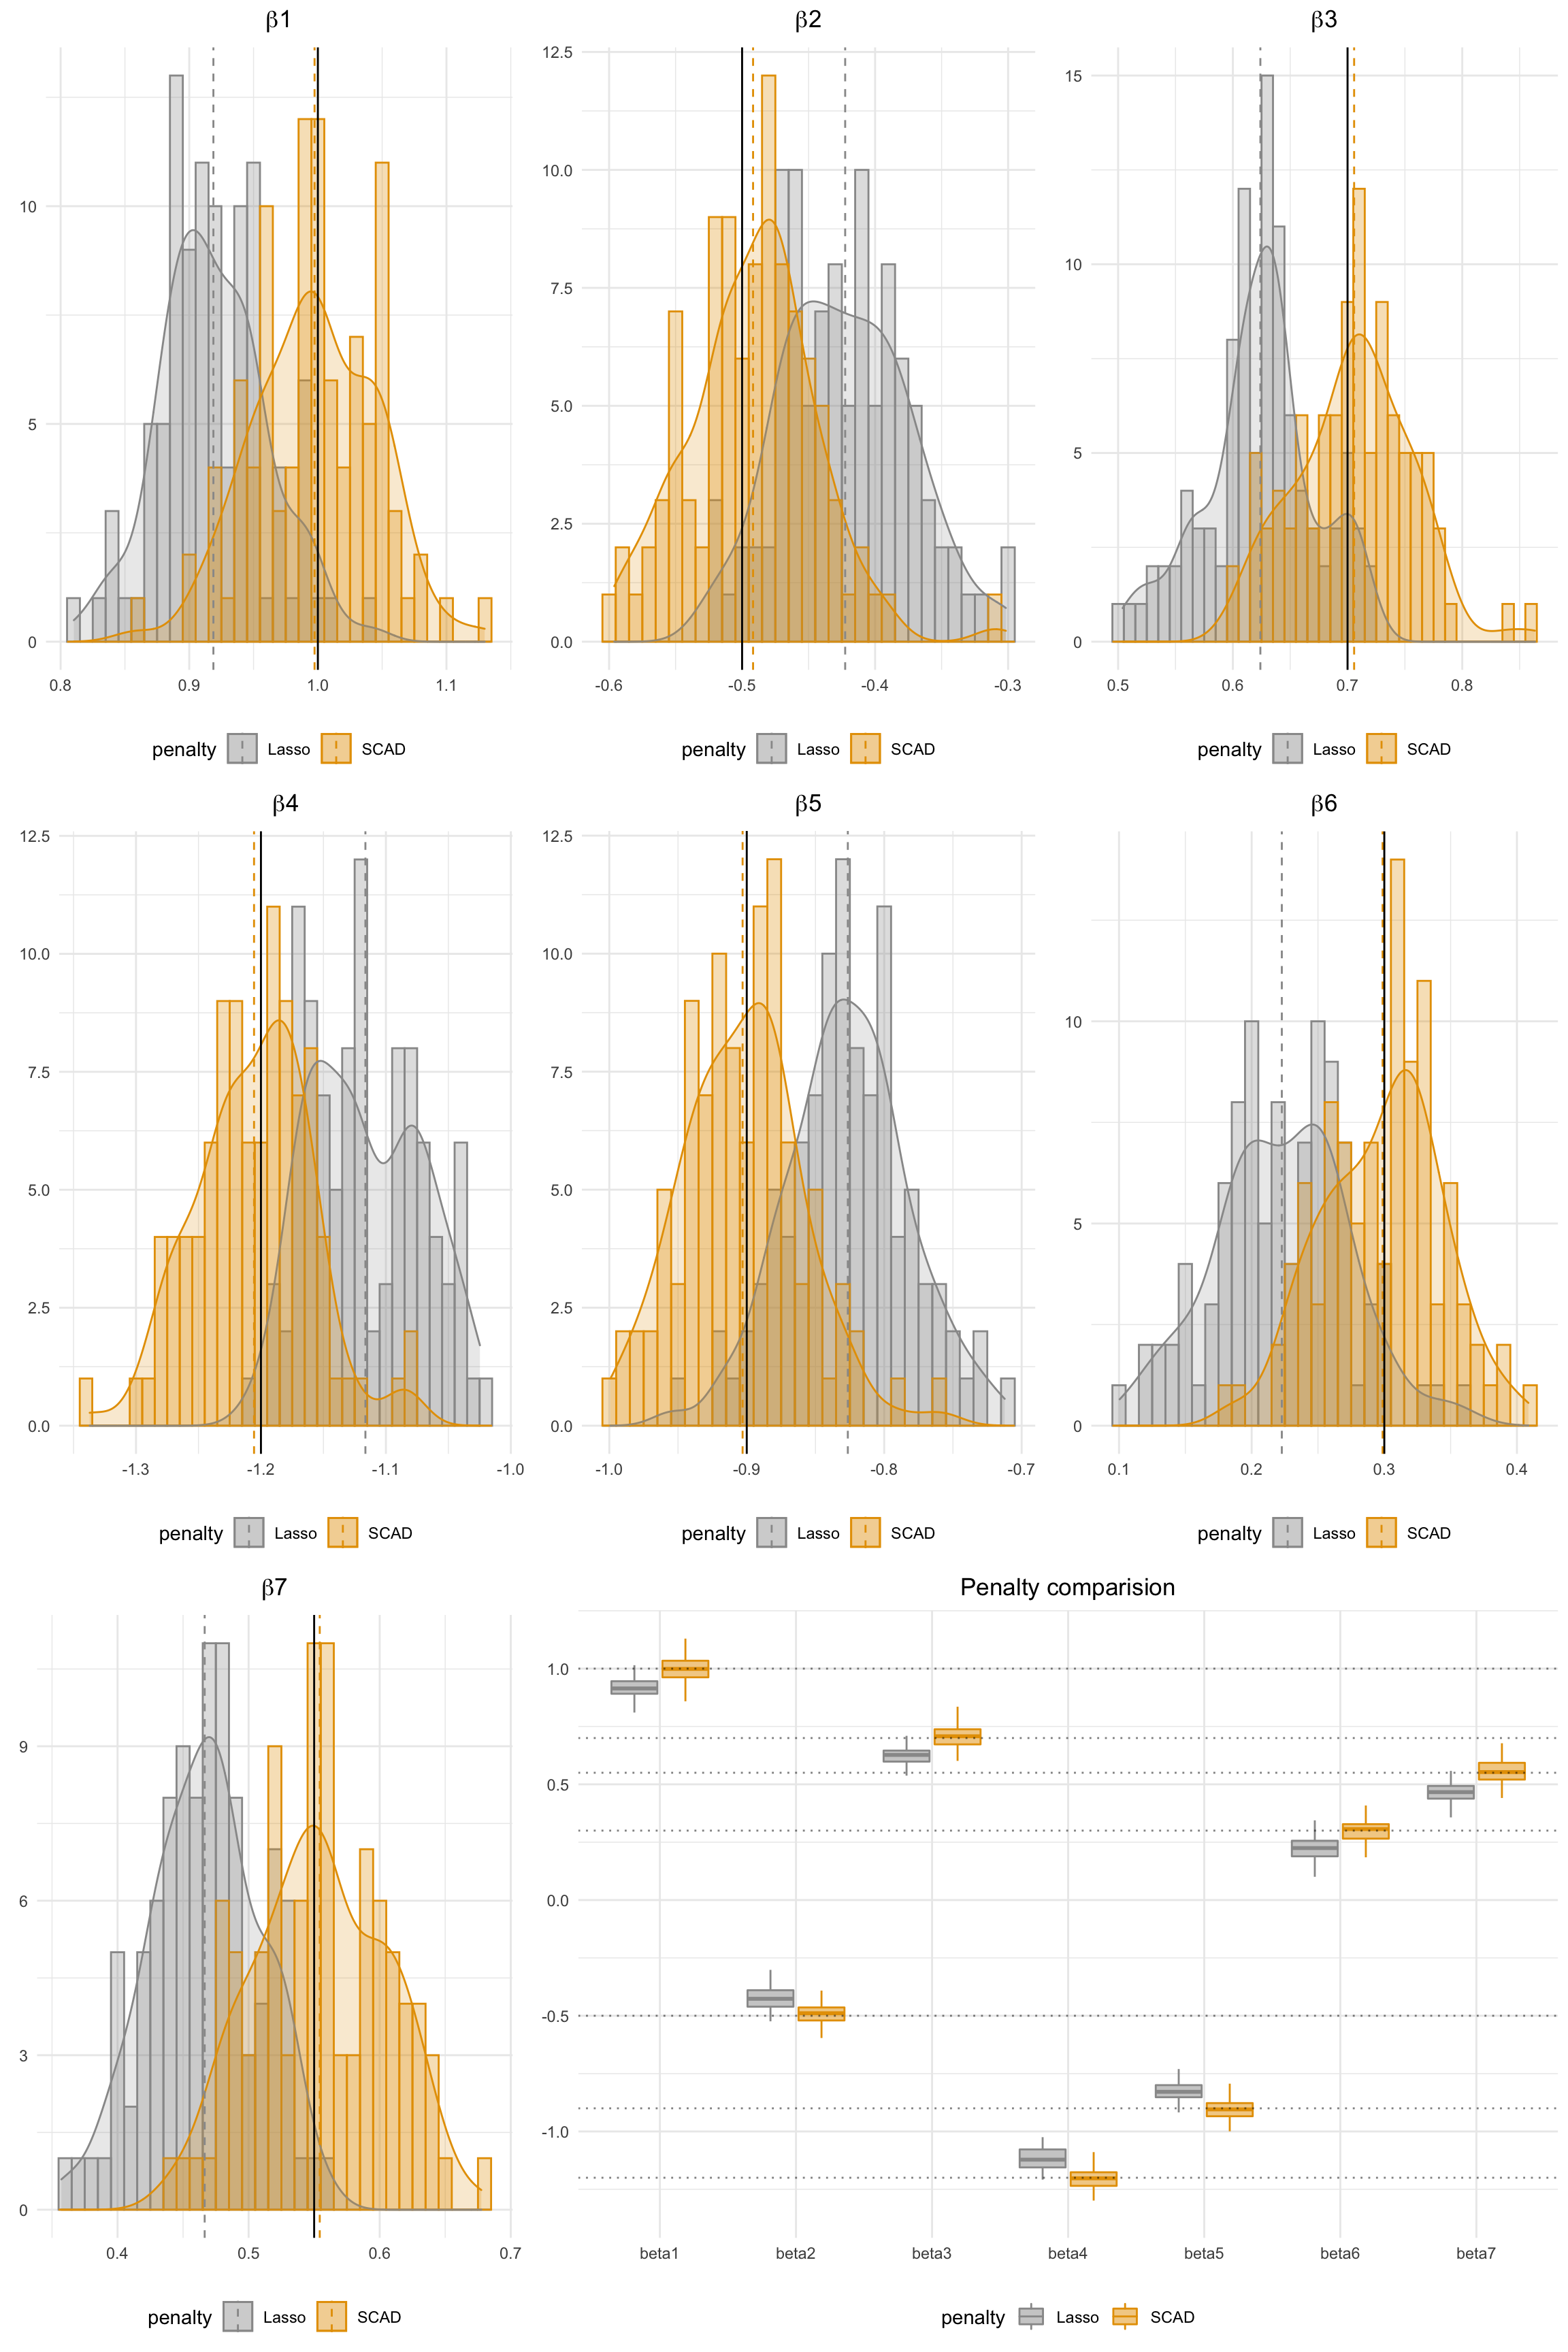
\includegraphics[width = 0.8 \textwidth]{figures/note12_SCADvsLasso.png}
\end{figure}

\newpage
\bibliographystyle{plainnat}
\bibliography{ref.bib}

\end{document}